%! suppress = MissingImport
%! suppress = MissingLabel
%! suppress = LineBreak

% CLI args https://tex.stackexchange.com/a/1501
\newif\ifhandout
\input{flags}

%! suppress = MissingLabel
%! suppress = DocumentclassNotInRoot
%! suppress = DiscouragedUseOfDef

% * Make friends tikz & colors
%   https://en.wikibooks.org/wiki/LaTeX/Colors
% * To enable vertical top alignment globally
%   https://tex.stackexchange.com/questions/9889/positioning-content-at-the-top-of-a-beamer-slide-by-default
% * Set handout from CLI
%   https://tex.stackexchange.com/a/1501
\ifhandout
\documentclass[usenames, dvipsnames, handout]{beamer} % https://tex.stackexchange.com/questions/224091/beamer-how-to-disable-pause-temporarily
\else
\documentclass[usenames, dvipsnames]{beamer}
\fi
% ------------------------------------------------

% Graphics
\usepackage{color}
\usepackage{tabularx}
\usepackage{tikz}
% https://tikz.dev/tikz-graphs
\usetikzlibrary{positioning, shapes.geometric, arrows, automata, graphs}
\tikzset{
    expr/.style={ellipse, draw=gray!60, fill=gray!5, very thick, minimum size=7mm, yshift=0.7cm},
    hexpr/.style={ellipse, draw=gray!60, fill=blue!15, very thick, minimum size=7mm, yshift=0.7cm},
    stmt/.style={rectangle, draw=gray!60, fill=gray!5, very thick, minimum size=5mm, yshift=0.7cm},
    decl/.style={rectangle, draw=blue!60, fill=gray!5, very thick, minimum size=5mm, yshift=0.7cm},
    hdecl/.style={rectangle, draw=blue!60, fill=blue!15, very thick, minimum size=5mm, yshift=0.7cm},
    subtree/.style={shape border rotate=90, isosceles triangle, draw=gray!60, fill=gray!5, very thick, minimum size=5mm, yshift=0.0cm},
}
\usepackage{blkarray}
\usepackage{graphicx}
\usepackage{forest} % https://tex.stackexchange.com/questions/198405/how-to-change-the-color-of-subtrees-in-tikz-qtree
% ------------------------------------------------

% Math
\usepackage{amsmath, amsfonts}
\usepackage{amssymb}
\usepackage{proof}
\usepackage{mathrsfs}
% Crossed-out symbols
% https://tex.stackexchange.com/questions/75525/how-to-write-crossed-out-math-in-latex
\usepackage[makeroom]{cancel}
\usepackage{mathtools}
% ------------------------------------------------

% Additional font sizes
% https://www.overleaf.com/learn/latex/Questions/How_do_I_adjust_the_font_size%3F
\usepackage{moresize}
% Additional colors
% https://www.overleaf.com/learn/latex/Using_colours_in_LaTeX
\usepackage{xcolor}
% Textual math symbols
\usepackage{textcomp}
% ------------------------------------------------

% Language
\usepackage[utf8] {inputenc}
\usepackage[T2A] {fontenc}
\usepackage[english, russian] {babel}
\usepackage{indentfirst, verbatim}
\usetikzlibrary{cd, babel}
% ------------------------------------------------

% Fonts: https://sites.math.washington.edu/~reu/docs/latex_symbols.pdf
\usepackage{stmaryrd}
\usepackage{cmbright}
\usepackage{wasysym}
\usepackage[weather]{ifsym} % https://tex.stackexchange.com/questions/100424/how-to-use-the-ifsym-package
% https://tex.stackexchange.com/questions/615300/pdflatex-builtin-glyph-names-is-empty
\pdfmapline{=dictsym DictSym <dictsym.pfb}
\pdfmapline{=pigpen <pigpen.pfa}
\usepackage{dictsym}
% ------------------------------------------------

% Code
% * Needs -shell-escape build flag
%   https://tex.stackexchange.com/questions/99475/how-to-invoke-latex-with-the-shell-escape-flag-in-texstudio-former-texmakerx
% * Set build directory
%   https://tex.stackexchange.com/questions/339931/latex-minted-package-using-custom-output-directory-build
\usepackage{minted}
\setminted{xleftmargin=\parindent, autogobble, escapeinside=\#\#}
% ------------------------------------------------

% Template
\usetheme{CambridgeUS}
\usecolortheme{dolphin}
% https://tex.stackexchange.com/questions/231439/beamer-how-to-make-font-larger-for-page-numbers
\setbeamerfont{headline}{size=\scriptsize}
\setbeamerfont{footline}{size=\scriptsize}
% Remove heddline
% https://tex.stackexchange.com/questions/33146/how-could-i-remove-a-header-in-a-beamer-presentation
%\setbeamertemplate{headline}{}
% Slide sizes
% https://tex.stackexchange.com/questions/56768/how-to-set-a-small-default-font-size-with-beamer
%\geometry{paperwidth=140mm,paperheight=105mm} % 4:3
\geometry{paperwidth=168mm,paperheight=105mm} % 16:10
% Remove navigation bar
% https://stackoverflow.com/questions/3210205/how-to-get-rid-of-navigation-bars-in-beamer
\beamertemplatenavigationsymbolsempty
% ------------------------------------------------

% Bullets
% https://9to5science.com/change-bullet-style-formatting-in-beamer
% https://tex.stackexchange.com/questions/185742/i-need-to-change-color-of-beamer-itemize-and-subitem-separately
\setbeamertemplate{itemize item}{\scriptsize\raise1.25pt\hbox{\donotcoloroutermaths$\blacktriangleright$}}
\setbeamertemplate{itemize subitem}{\scriptsize\raise1.5pt\hbox{\donotcoloroutermaths$\blacktriangleright$}}
\setbeamertemplate{itemize subsubitem}{\tiny\raise1.5pt\hbox{\donotcoloroutermaths$\blacktriangleright$}}
\setbeamertemplate{enumerate item}{\insertenumlabel.}
\setbeamertemplate{enumerate subitem}{\insertenumlabel.\insertsubenumlabel}
\setbeamertemplate{enumerate subsubitem}{\insertenumlabel.\insertsubenumlabel.\insertsubsubenumlabel}
% ------------------------------------------------

% Table of contents format
% https://tex.stackexchange.com/questions/642927/format-table-of-contents-in-beamer
\setbeamertemplate{section in toc}{%
        {\color{blue}\inserttocsectionnumber.}
    \inserttocsection\par%
}
\setbeamertemplate{subsection in toc}{%
        {\color{blue}\hspace{1em}\scriptsize\raise1.25pt\hbox{\donotcoloroutermaths$\blacktriangleright$}}
    \inserttocsubsection\par%
}
\setbeamertemplate{subsubsection in toc}{%
        {\color{blue}\hspace{2em}\tiny\raise1.25pt\hbox{\donotcoloroutermaths$\blacktriangleright$}}
    \inserttocsubsubsection\par%
}
% ------------------------------------------------

% Misc
\usepackage{multicol}
\usepackage{hyperref}
\usepackage{soul} % https://tex.stackexchange.com/questions/23711/strikethrough-text
% ------------------------------------------------

% Fix \pause for amsmath package envs (black black magic)
% https://tex.stackexchange.com/questions/16186/equation-numbering-problems-in-amsmath-environments-with-pause/75550#75550
% https://tex.stackexchange.com/questions/6348/problem-with-beamers-pause-in-alignments
%! suppress = Makeatletter
\makeatletter
\let\save@measuring@true\measuring@true
\def\measuring@true{%
    \save@measuring@true
    \def\beamer@sortzero##1{\beamer@ifnextcharospec{\beamer@sortzeroread{##1}}{}}%
    \def\beamer@sortzeroread##1<##2>{}%
    \def\beamer@finalnospec{}%
}
%! suppress = Makeatletter
\makeatother
% ------------------------------------------------

% Sections
\newcommand{\sectionplan}[1]{\section{#1}%
    \begin{frame}[noframenumbering]{Содержание}
        \tableofcontents[currentsection]
    \end{frame}
}
\newcommand{\subsectionplan}[1]{\subsection{#1}%
    \begin{frame}[noframenumbering]{Содержание}
        \tableofcontents[currentsubsection]
    \end{frame}
}
% ------------------------------------------------

% Footnotes
\renewcommand{\thefootnote}{\arabic{footnote}}
\renewcommand{\thempfootnote}{\arabic{mpfootnote}}
% https://tex.stackexchange.com/questions/28465/multiple-footnotes-at-one-point
\usepackage{fnpct}
% ------------------------------------------------

% Links
% Colors also links on slide foot.
%\hypersetup{
%    colorlinks=true,
%    citecolor=blue,
%    linkcolor=blue,
%    urlcolor=blue
%}
% ------------------------------------------------

% Appendix
% Slide numbers
% https://tex.stackexchange.com/questions/70448/dont-count-backup-slides
\usepackage{appendixnumberbeamer}
\newcommand{\backupbegin}{
    \newcounter{framenumbervorappendix}
    \setcounter{framenumbervorappendix}{\value{framenumber}}
}
\newcommand{\backupend}{
    \addtocounter{framenumbervorappendix}{-\value{framenumber}}
    \addtocounter{framenumber}{\value{framenumbervorappendix}}
}
% ------------------------------------------------

% Custom commands
% * Decor
\newcommand{\newtopic}[0]{$+$} % item: new topic on "in previous series"
\newcommand{\then}{$\Rightarrow$} % item: consequences
\newcommand{\pop}[0]{\SunCloud} %item:  general eduation
\newcommand{\popslide}[0]{(\pop)}
\newcommand{\advanced}[0]{$\varhexstar$} % item: advanced science
\newcommand{\advancedslide}[0]{(\advanced)}
\newcommand{\practical}[0]{\dstechnical} % item: practical programming notions
\newcommand{\practicalslide}[0]{(\practical)}
\newcommand{\todo}[0]{todo} % item: question
\newcommand{\answer}[0]{\Lightning} % item: answer to the previous question
\newcommand{\eg}[0]{e.g.} % item: example
\newcommand{\defi}[0]{$\Delta$} % item: definition on smth
\newcommand{\textdefi}[1]{\textbf{#1}}
\newcommand{\positive}{$+$} % item: pros
\newcommand{\negative}{{\color{red} $-$}} % item: cons
\newcommand%! suppress = EscapeHashOutsideCommand
\NB[1][0.3]{N\kern-#1em{B}} % default kern amount: -0.3em
\renewcommand{\emph}[1]{{\color{blue} \textit{#1}}}
\newcommand{\vocab}[1]{\textbf{#1}} % item: important new word
% * Lambda calculi
\newcommand{\comb}[1]{\mathbf{#1}} % defined combinator
\newcommand{\term}[1]{\mathbf{#1}} % predefined lambda-term reference
\newcommand{\termdef}{\coloneqq} % lamda term binding
\newcommand{\step}{\rightsquigarrow} % reduction step
\newcommand{\sstep}{\twoheadrightarrow} % multiple steps reduction
\newcommand{\ap}{~} % lambda-term application
\newcommand{\subst}[3]{\left[#2 \mapsto #3 \right] #1} % substitution
\newcommand{\eqbeta}{=_\beta} % beta equality
\newcommand{\eqeta}{=_\eta} % eta-equality
\newcommand{\eqt}{=} % tree-equality of terms
\newcommand{\tlist}[1]{\term{[}#1\term{]}} % list-term
% * Legacy
%\newcommand{\err}[0]{\textcolor{red}{ошибка}} % compilation error

% ------------------------------------------------

% Speaker notes
% https://tex.stackexchange.com/questions/114219/add-notes-to-latex-beamer
% https://tex.stackexchange.com/questions/35444/split-beamer-notes-across-multiple-notes-pages/35496#35496
%\setbeameroption{show notes on second screen=right} % enable speaker notes
%--------------------------------------

\author[]{Андрей Стоян, Илья Колегов, Дмитрий Халанский}
\institute[MSE ITMO]{MSE ITMO}

\setminted{xleftmargin=\parindent, autogobble, escapeinside=??}

\title[3. Ad-hoc полиморфизм]{3. Ad-hoc полиморфизм}
\author{Андрей Стоян}
\institute[ИПКН ИТМО]{ИПКН ИТМО}

\date{осень 2025}

\begin{document}

    \mymaketitle

    \begin{frame}[noframenumbering]{Содержание}
        \tableofcontents
    \end{frame}

    \begin{frame}[fragile]{Классы типов и перегрузка}
        \pause
        \begin{minted}{cpp}
            string toString(x: int) { ... }
            string toString(fmt: String, d: double) { ... }
        \end{minted}
        \pause\vspace{1em}
        \begin{minted}{haskell}
            class Show a where
              show :: a -> String

            instance Show Int where
              show :: Int -> String
              show = ...
        \end{minted}
        \pause\vspace{1em}
        \begin{minted}{haskell}
            showPrefixed :: Show a => a -> String -> String
        \end{minted}
    \end{frame}

    \sectionplan{Классы типов в языке}

    \begin{frame}[fragile]{Словари}
        \pause
        \begin{minted}{haskell}
            data OrdDict a = OrdDict { less :: a -> a -> Bool }

            sort :: OrdDict a -> [a] -> [a]
            sort d@OrdDict { less } = \case [] -> []; x:xs -> insert x (sort d xs)
              where
                insert x xs = let (l, r) = List.partition (?\framebox{`less`}? x) xs in l ++ x : r
        \end{minted}
    \end{frame}

    \begin{frame}[fragile]{}
        \pause
        \begin{minted}{haskell}
            intOrd :: OrdDict Int
            intOrd = OrdDict { less = (<) }

            ghci> sort intOrd [3, 2, 1]
        \end{minted}
        \pause\vspace{1em}
        \begin{minted}{haskell}
            listDict :: OrdDict a -> OrdDict [a]
            listDict d = OrdDict { less = ... ?\framebox{less d}? ... }
        \end{minted}
        \pause\vspace{1em}
        \begin{minted}{haskell}
            ghci> sort (listDict intDict) [[3, 2], [2, 1], [0]]
        \end{minted}
    \end{frame}

    \begin{frame}[fragile]{Type-directed translation}
        \begin{tabular}{p{7cm}p{7cm}}
            \begin{enumerate}
                \item Определение словаря функций
                \begin{minted}{haskell}
            data MyOrd a = MyOrd
              { less :: a -> a -> Bool }
                \end{minted}
                \item Экземпляр словаря для конкретного типа
                \begin{itemize}
                    \item Именованное значение
                \end{itemize}
                \begin{minted}{haskell}
            intMyOrd :: MyOrd Int
            intMyOrd = MyOrd { less = (<) }
                \end{minted}
                \item Явный параметр функции
                \begin{minted}{haskell}
            sort :: MyOrd a -> [a] -> [a]
                \end{minted}
                \item Передаётся пользователем
                \begin{minted}{haskell}
            test = sort ?\framebox{intMyOrd}? [3, 2, 1]
                \end{minted}
            \end{enumerate}
            &
            \begin{enumerate}
                \item Определение класса типов
                \begin{minted}{haskell}
             class MyOrd a where
               less :: a -> a -> Bool
                \end{minted}
                \item Объявление типа представителем класса типов
                \begin{itemize}
                    \item Не имеет имени
                \end{itemize}
                \begin{minted}{haskell}
            instance MyOrd Int where
              less = (<)
                \end{minted}
                \item Неявный параметр функции
                \begin{minted}{haskell}
            sort :: MyOrd a => [a] -> [a]
                \end{minted}
                \item Передаётся компилятором
                \begin{minted}{haskell}
            test = sort [3, 2, 1]
                \end{minted}
            \end{enumerate}
        \end{tabular}
    \end{frame}

    \begin{frame}[fragile]{Неявные аргументы}
        \pause
        \begin{minted}{haskell}
            f :: (Show b => b) -> b
            f x = ?\framebox{x}?
        \end{minted}
        \pause\vspace{1em}
        \begin{minted}{haskell}
            f :: Show b => (Show b => b) -> b
            f x = ?\framebox{x}?
        \end{minted}
        \pause\vspace{1em}
        \begin{minted}[escapeinside=##]{haskell}
            sortBy :: (a -> a -> Bool) -> [a] -> [a]

            sort :: (?cmp :: a -> a -> Bool) => [a] -> [a]
            sort = sortBy ?cmp
        \end{minted}
        \pause\vspace{1em}
        \begin{minted}{haskell}
            data ShowDict a where
              ShowDict :: Show a => ShowDict a

            f :: ShowDict b -> (Show b => b) -> b
            f d x = case d of ShowDict -> ?\framebox{x}? -- в скоупе доступен инстанс Show b
        \end{minted}
    \end{frame}

    \begin{frame}[fragile]{Вывод инстансов}
        \pause
        \begin{minted}{haskell}
            type data Nat = Zero | Suc Nat

            class KnownNat (n :: Nat) where
              natVal :: Int

            instance KnownNat Zero where
              natVal = 0

            instance KnownNat n => KnownNat (Suc n) where
              natVal = 1 + natVal @n

            ghci> natVal @(Suc (Suc Zero))
            -- выведется natVal {knownSuc (knownSuc knownZero)}
        \end{minted}
    \end{frame}

    \begin{frame}[fragile]{Вычисления на тайпклассах}
        \pause
        \begin{minted}{haskell}
            class Reverse (acc :: [Type]) (tys :: [Type]) where
              showReverse :: String

            instance ShowT acc => Reverse acc '[] where
              showReverse = showTypes @acc

            instance Reverse (ty : acc) tys => Reverse acc (ty : tys) where
              showReverse = showReverse @(ty : acc) @tys

            ghci> showReverse @'[] @'[Char, Int, Double]
        \end{minted}
    \end{frame}

    \begin{frame}[fragile]{Классы типов и кодогенерация}
        \begin{figure}[h]
            \centering
            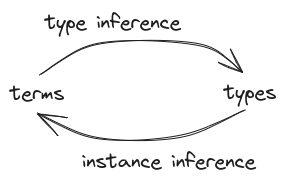
\includegraphics[width=0.4\textwidth]{figs/class-sinergy}
            \caption{Классы типов + вывод инстансов = кодогенерация.}
            \label{fig:class-sinergy}
        \end{figure}
    \end{frame}

    \begin{frame}[fragile]{Построение типа по значению}
        \pause
        \begin{minted}{haskell}
            reify :: Int -> (forall n. KnownNat n => a) -> a
            reify n k
              | n <= 0 = k @Zero
              | otherwise = reify (n - 1) \@n' -> k @(Suc n')
        \end{minted}
        \pause\vspace{1em}
        \begin{minted}{haskell}
            wonderId :: Int -> Int
            wonderId n = reify n (\@t -> natVal @t)
        \end{minted}
    \end{frame}

    \begin{frame}[fragile]{Классы типов через имплиситы}
        \pause
        \begin{minted}{scala}
            // Пачка функций.
            trait Show[T] {
                def show(x: T): String
            }

            // Обёртка для удобства вызова.
            def show[T](x: T)(implicit ev: Show[T]): String = ev.show(x)

            // Объект-синклтон, значение для пачки функций.
            implicit object intShow extends Show[Int] {
                def show(x: Int): String = x.toString
            }

            def showAll[T](xs: List[T])(implicit ev: Show[T]): String =
                xs.map(show(_)).join(", ")
        \end{minted}
    \end{frame}

    \begin{frame}[fragile]{Когерентность инстансов}
        \begin{figure}
            \centering
            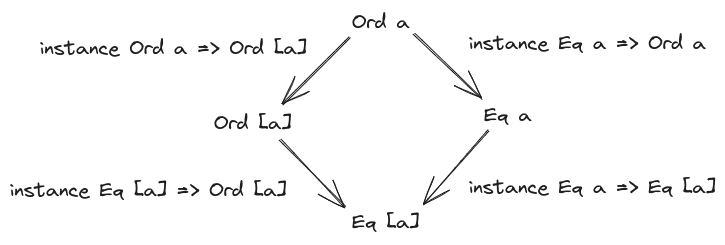
\includegraphics[width=0.8\linewidth]{figs/coherence}
            \caption{Когерентность инстансов --- диаграмма коммутирует.}
            \label{fig:coherence}
        \end{figure}
    \end{frame}

    \begin{frame}[fragile]{Правила (rules) и специализация}
        \pause
        \begin{minted}{haskell}
            {-# RULES
              "map/map"    forall f g xs.  map f (map g xs) = map (f . g) xs
              "map/append" forall f xs ys. map f (xs ++ ys) = map f xs ++ map f ys
             #-}
        \end{minted}
        \pause\vspace{1em}
        \begin{minted}{haskell}
            genericLookup :: Ord a => Table a b   -> a   -> b
            intLookup     ::          Table Int b -> Int -> b

            {-# RULES "genericLookup/Int" genericLookup = intLookup #-}
        \end{minted}
    \end{frame}

    \begin{frame}[fragile]{Отступление: дефункционализация}
        \pause
        \begin{minted}{haskell}
            map :: (Int -> Int) -> [Int] -> [Int]
            map f = \case [] -> []; x:xs -> f x : map f xs

            example1 xs = map (\x -> x + 1) xs
            example2 y xs = map (\x -> x * y) xs
        \end{minted}
        \pause\vspace{1em}
        \begin{minted}{haskell}
            data Fun = F1 | F2 Int
            apply :: Fun -> Int -> Int
            apply df x = case df of F1 -> x + 1; F2 y -> x + y

            map :: Fun -> [Int] -> [Int]
            map df = \case [] -> []; x:xs -> apply df x : map df xs

            example1 xs = map F1 xs
            example2 y xs = map (F2 y) xs
        \end{minted}
    \end{frame}

    \begin{frame}[fragile]{Эмуляция полиморфизма высших порядков}
        \pause
        \begin{minted}{kotlin}
            class ListSym
        \end{minted}
        \pause
        \begin{minted}{kotlin}
            class Apply<Sym, T>(val value: Any)
        \end{minted}
        \pause
        \begin{minted}{kotlin}
            fun <T> List<T>.to(): Apply<ListSym, T> = Apply(this)
            fun <T> Apply<ListSym, T>.from(): List<T> = this.value as List<T>
        \end{minted}
        \pause
        \begin{minted}{kotlin}
            interface Monad<M> {
                fun <T> pure(x: T): Apply<M, T>
                infix fun <T, R> Apply<M, T>.bind(k: (T) -> Apply<M, R>): Apply<M, R>
            }
            object ListMonad : Monad<ListSym> {
                override fun <T> pure(x: T): Apply<ListSym, T> = listOf(x).to()
                override fun <T, R> Apply<ListSym, T>.
                        bind(k: (T) -> Apply<ListSym, R>): Apply<ListSym, R> =
                    this.from().flatMap { k(it).from() }.to()
            }
        \end{minted}
        \pause
        \begin{minted}{kotlin}
            fun <M> Monad<M>.go(x: Apply<M, Int>): Apply<M, Int> =
                x bind { it -> pure(it + 1) } bind { it -> pure(it + 2) }
            fun test(xs: List<Int>): List<Int> = ListMonad.go(xs.to()).from()
        \end{minted}
    \end{frame}

    \sectionplan{Семейства}

    \begin{frame}[fragile]{Data families}
        \pause
        \begin{minted}{haskell}
            data family XList elem
            data instance XList () = IntList Int
            data instance XList Bool = BoolList ByteArray
        \end{minted}
        \pause\vspace{1em}
        \begin{minted}{haskell}
            class XListOp elem where
              xelem :: elem -> XList elem -> Bool

            instance XListOp () where
              xelem () (IntList size) = size > 0

            instance XList Bool where
              xelem key (ByteArray bs) = ...

            xelemAll :: XListOp elem => XList elem -> [elem] -> Bool
            xelemAll xs = all (`xelem` xs)
        \end{minted}
    \end{frame}

    \begin{frame}[fragile]{Synonym families}
        \pause
        \begin{minted}{haskell}
            type family Plus (n :: Nat) (m :: Nat) :: Nat where
              Plus Zero m = m
              Plus (Suc n) m = Suc (Plus n m)
        \end{minted}
        \pause\vspace{1em}
        \begin{minted}{haskell}
            ghci> :k! Plus (Suc Zero) (Suc (Suc Zero))
            Plus (Suc Zero) (Suc (Suc Zero)) :: Nat
            = Suc (Suc (Suc Zero))
        \end{minted}
    \end{frame}

    \begin{frame}[fragile]{Ассоциированные семейства}
        \pause
        \begin{minted}{haskell}
            class Container a where
              type Elem a
              elements :: a -> [Elem a]

            instance Container [a] where
              type Elem [a] = a
              elements = id

            instance Container ByteString where
              type Elem ByteString = Word8
              elements = ByteString.unpack
        \end{minted}
    \end{frame}

    \begin{frame}[fragile]{Инъективные семейства}
        \pause
        \begin{minted}{haskell}
            Maybe a ?$\sim$? Maybe b ?$\Rightarrow$? a ?$\sim$? b
        \end{minted}
        \pause\vspace{1em}
        \begin{minted}{haskell}
            type family NonInjective a where
              NonInjective Int = Double
              NonInjective Char = Double
        \end{minted}
        \pause\vspace{1em}
        \begin{minted}{haskell}
            type family InjectiveB a b = r | r -> b
              ...
        \end{minted}
    \end{frame}

    \begin{frame}[fragile]{Семейства первого класса}
        \pause
        \begin{minted}{haskell}
            f a ?$\sim$? g a ?$\Rightarrow$? f ?$\sim$? g
        \end{minted}
        \pause\vspace{1em}
        \begin{minted}{haskell}
            type family ToCtor (s :: Symbol) :: Type -> Type where
              ToCtor "maybe" = Maybe
              ToCtor "identity" = Identity
        \end{minted}
        \pause\vspace{1em}
        \begin{minted}{haskell}
            data Matchability = Matchable | Unmatchable

            hMap
              :: forall (m :: Matchability) (c :: Type -> Constraint)
               . forall (f :: Type ->?$^m$? Type) (as :: [Type])
               . All as c => (forall a. c a => a -> f a) -> HList as -> HList (Map f as)
        \end{minted}
    \end{frame}

    \sectionplan{Кайнд \texttt{Constraint}}

    \begin{frame}[fragile]{Кайнд \texttt{Constraint}}
        \pause
        \begin{itemize}
            \item Класс типов конструирует констреинт: \mintinline{haskell}|Monad :: (Type -> Type) -> Constraint|;
            \item Эквивалентность является констреинтом: \mintinline{haskell}|(a ?$\sim$? b) :: Constraint|;
            \item Пустой кортеж констреинтов является констреинтом: \mintinline{haskell}|() :: Constraint|;
            \item Кортеж констреинтов является констреинтом: \mintinline{haskell}|(Eq a, a ?$\sim$? b) :: Constraint|.
        \end{itemize}
        \pause\vspace{1em}
        \begin{minted}{haskell}
            data Dict (c :: Constraint) where
              Dict :: c => Dict c
        \end{minted}
    \end{frame}

    \begin{frame}[fragile]{Вариадики своими руками}
        \pause
        \begin{minted}{haskell}
            data HList (tys :: [Type]) where
              HNil :: HList '[]
              HCons :: ty -> HList tys -> HList (ty : tys)
        \end{minted}
        \pause\vspace{1em}
        \begin{minted}{haskell}
            type family All (c :: k -> Constraint) (tys :: [k]) :: Constraint where
              All c '[] = ()
              All c (ty : tys) = (c ty, All c tys)

            -- All Show [Int, Double] ?$\sim$? (Show Int, (Show Double, ())
        \end{minted}
        \pause\vspace{1em}
        \begin{minted}{haskell}
            hmap :: forall c res tys . All c tys
                 => (forall ty . c ty => ty -> res) -> HList tys -> [res]
            hmap f = \case
              HNil -> []
              HCons x xs -> f x : hmap @c f xs

            ghci> hmap @Show show (HCons (1 :: Int) $ HCons 'a' HNil)
        \end{minted}
    \end{frame}

    \begin{frame}[fragile]{Полиморфные констреинты}
        \pause
        \begin{minted}{haskell}
            data Rose f x = Rose x (f (Rose f x))

            instance (Eq a, forall b. Eq b => Eq (f b)) => Eq (Rose f a) where
              Rose x1 rs1 == Rose x2 rs2 = x1 == x2 && rs1 == rs2
        \end{minted}
    \end{frame}

    \sectionplan{Использование ad-hoc полиморфизма}

    \begin{frame}[fragile]{Сериализация}
        \pause
        \begin{minted}{kotlin}
            interface KSerializer<T> {
                fun serialize(encoder: Encoder, value: T)
                fun deserialize(decoder: Decoder): T
            }
        \end{minted}
        \pause\vspace{1em}
        \begin{minted}{kotlin}
            class PairSerializer(
                keySerializer: KSerializer<K>,
                valueSerializer: KSerializer<V>,
            ): KSerializer<Pair<K, V>> { ... }
        \end{minted}
    \end{frame}

    \begin{frame}[fragile]{Экзистенциальные типы}
        \pause
        \begin{minted}{haskell}
            data Any where
              Any :: forall a . a -> Any  -- логически эквивалентно (exists a . a) -> Any

            list :: [Any]
            list = [Any 42, Any "Hello", Any (Just Nothing)]
        \end{minted}
        \pause\vspace{1em}
        \begin{minted}{haskell}
            data Has (c :: Type -> Constraint) where
              Has :: c a => a -> Has c
        \end{minted}
        \pause\vspace{1em}
        \begin{minted}{haskell}
            showAll :: [Has Show] -> String
            showAll = List.intercalate "," . map \(Has x) -> show x
        \end{minted}
        \pause\vspace{1em}
        \begin{minted}{haskell}
            foldHas :: Has c -> (forall a . c a => a -> b) -> b
            foldHas (Has x) k = k x
        \end{minted}
    \end{frame}

    \begin{frame}[fragile]{Разрешение имён}
        \pause
        \begin{minted}{haskell}
            class IsLabel (s :: Symbol) a where
              fromLabel :: a
        \end{minted}
        \pause\vspace{1em}
        \begin{minted}{haskell}
            #name ?$\equiv$? fromLabel @"name"
        \end{minted}
        \pause\vspace{1em}
        \begin{minted}{haskell}
            data Pet = Pet { name :: String }
            instance IsLabel "name" (Pet -> String) where
              fromLabel Pet{ name } = name

            data Person = Person { name :: String, pets :: [Pet] }
            instance IsLabel "name" (Person -> String) where
              fromLabel Person{ name } = name

            ghci> #name pet
        \end{minted}
    \end{frame}

    \begin{frame}[fragile]{Несинтаксические типовые эквивалентности, System FC}
        \pause
        \begin{minted}{haskell}
            f :: forall a b . a ?$\sim$? b => a -> b
            f = id
        \end{minted}
        \pause\vspace{1em}
        \begin{minted}{haskell}
            data Expr ty where
              Const :: Int -> Expr Int
              IsZero :: Expr Int -> Expr Bool
              If :: forall ty . Expr Bool -> Expr ty -> Expr ty -> Expr ty
            -- транслируется в
            data Expr ty where
              Const :: forall ty . ty ?$\sim$? Int => Expr ty
              IsZero :: forall ty . ty ?$\sim$? Bool => Expr Int -> Expr ty
              If :: forall ty . Expr Bool -> Expr ty -> Expr ty -> Expr ty
        \end{minted}
    \end{frame}

    \begin{frame}[fragile]{Трансляция семейств}
        \pause
        \begin{minted}{haskell}
            type family Plus (n :: Nat) (m :: Nat) :: Nat where
              Plus Zero m = m
              Plus (Suc n) m = Suc (Plus n m)
            -- раскроется в
            axiom Plus Zero m ?$\sim$? m
            axiom Plus (Suc n) m ?$\sim$? Suc (Plus n m)
        \end{minted}
    \end{frame}

    \begin{frame}[fragile]{Коерции и роли}
        \pause
        \begin{minted}{haskell}
            newtype ModuleId = ModuleId Int64
            newtype CourceId = CourceId Int64
        \end{minted}
        \pause\vspace{1em}
        \begin{minted}{haskell}
            newtype Csv = Csv { unCsv :: String }

            concatC :: [Csv] -> Csv
            concatC = Csv . concat . ?\framebox{map}? unCsv
        \end{minted}
        \pause\vspace{1em}
        \begin{minted}{haskell}
            class Coercible from to where
              coerce :: from -> to
        \end{minted}
        \pause\vspace{1em}
        \begin{minted}{haskell}
            concatC :: [Csv] -> Csv
            concatC = coerce concat
        \end{minted}
        \pause\vspace{1em}
        \begin{minted}{haskell}
            type role Map nominal representational
            data Map k v = ...
        \end{minted}
    \end{frame}

    \begin{frame}[fragile]{Type reflection}
        \pause
        \begin{minted}{haskell}
            class Typeable a where
              typeRep :: TypeRep a
        \end{minted}
        \pause\vspace{1em}
        \begin{minted}{haskell}
            typeName :: forall a. Typeable a => String
            typeName = tyConName $ typeRepTyCon $ typeRep $ Proxy @a

            ghci> typeName @Int
        \end{minted}
        \pause\vspace{1em}
        \begin{minted}{haskell}
            data Dynamic where
              Dynamic :: Typeable a => a -> Dynamic

            fromDynamic :: Typeable a => Dynamic -> Maybe a
        \end{minted}
        \pause\vspace{1em}
        \begin{minted}{haskell}
            data Store = Map Key Dynamic
            data Ref ty = Ref Key
            get :: Typeable ty => Store -> Ref ty -> Maybe ty
        \end{minted}
    \end{frame}

    \begin{frame}[fragile]{Data reflection}
        \pause
        \begin{minted}{haskell}
            class Reifies ty terms | ty -> terms where
              reflect :: Proxy ty -> terms
        \end{minted}
        \pause\vspace{1em}
        \begin{minted}{haskell}
            reify :: a -> (forall fresh . Reifies fresh a => Proxy fresh -> res) -> res
        \end{minted}
        \pause\vspace{1em}
        \begin{minted}{haskell}
            newtype Wrapped tag a = Wrapped { unwrap :: a }
        \end{minted}
        \pause\vspace{1em}
        \begin{minted}{haskell}
            data ReifiedOrd a = ReifiedOrd { compare :: a -> a -> Ordering }

            instance Reifies tag (ReifiedOrd a) => Ord (Wrapped tag a) where
              compare = coerce $ compare $ reflect $ Proxy @tag
        \end{minted}
    \end{frame}

    \begin{frame}[fragile]{Использование data reflection}
        \pause
        \begin{minted}{haskell}
            sort :: Ord a => [a] -> [a]

            sortReverse :: forall a . Ord a => [a] -> [a]
            sortReverse xs =
              let dict = ReifiedOrd { compare = flip compare } in
              reify dict \(Proxy :: Proxy fresh) ->
                coerce $ sort @(Wrapped fresh a) $ coerce xs
        \end{minted}
    \end{frame}

    \begin{frame}[fragile]{Открытые структуры}
        \pause
        \begin{minted}{haskell}
            (Int, Double) ?заменяем на? (Member Int d, Member Double d) => Prod d
        \end{minted}
    \end{frame}

    \begin{frame}[fragile]{Легковесные частичные стек-трейсы}
        \pause
        \begin{minted}{haskell}
            myHead :: HasCallStack => [a] -> a
            myHead []     = error "empty"
            myHead (x:xs) = x

            bad :: Int
            bad = myHead []

            ghci> bad
            *** Exception: empty
            CallStack (from HasCallStack):
              error, called at Bad.hs:8:15 in main:Bad
              myHead, called at Bad.hs:12:7 in main:Bad
              -- no information about bad call site here
        \end{minted}
        \pause\vspace{1em}
        \begin{minted}[escapeinside=##]{haskell}
            type HasCallStack = (?callStack :: CallStack)
        \end{minted}
    \end{frame}

    \begin{frame}[fragile]{Кастомизируемые ошибки типизации}
        \pause
        \begin{minted}{haskell}
            instance (TypeError
              ( Text "Attempting to show a function of type "
                :<>: Text "'" :<>: ShowType (a -> b) :<>: Text "'"
                :$$: Text "Did you forget to apply an argument?"
              )) => Show (a -> b) where
              show = undefined -- реализация не важна, до исполнения дело не дойдёт
        \end{minted}
    \end{frame}

\end{document}
